\documentclass[12pt,a4paper]{extreport}
\usepackage{epsfig}
\usepackage{moreverb}
\usepackage{color}
\usepackage{fancyhdr,a4wide}
\usepackage{makeidx}
\usepackage{amssymb,amsmath}
\usepackage{multirow}
\usepackage{fancyvrb}
\usepackage{listings} 
\usepackage[ngerman,english]{babel}
\usepackage{graphicx}
\usepackage{url}
\usepackage[pdffitwindow=true,pdfstartview=Fit]{hyperref}
\usepackage{amssymb,amsmath}
\usepackage[nonumberlist,acronym,toc]{glossaries}
\usepackage[all]{hypcap}

\makeglossaries
\newacronym{IR}{IR}{Information Retrieval}
\newacronym{LSA}{LSA}{Latent Semantic Analysis}
\newacronym{CMS}{CMS}{Content Management Systems}
\newacronym{LSI}{LSI}{Latent Semantic Indexing}
\newacronym{SVD}{SVD}{Singular Value Decomposition}
\newacronym{VSM}{VSM}{Vector Space Model}


% don't indent new paragraphs
\parindent 0pt

\hoffset+0.3in
\textwidth13cm
\textheight22cm

\usepackage{graphicx}
\makeatletter
\def\ScaleIfNeeded{%
\ifdim\Gin@nat@width>\linewidth
\linewidth
\else
\Gin@nat@width
\fi
}
\makeatother

\pagestyle{headings}
\begin{document}
\clubpenalty = 10000
\widowpenalty = 10000 
\displaywidowpenalty = 10000

\newenvironment{summary}{\begin{quotation}\it\textbf{Summary.\space}}{\end{quotation}\vspace{0.3cm}}
\begin{titlepage}
\begin{minipage}{1\linewidth}
\begin{flushright}
\begin{minipage}[h]{0.4\linewidth}

\includegraphics[height=2cm]{img/STSlogo}
\end{minipage}
\hspace{0.5cm}
\begin{minipage}[h]{0.4\linewidth}

\includegraphics[height=2cm]{img/CoremediaLogo}
\end{minipage}\\
\bigskip
\Huge
\hrulefill\\
\bigskip
Tag Cloud Control \\by Latent Semantic Analysis\\
\hrulefill\\ \bigskip \bigskip
\normalsize submitted by\\
\large
Angelina Velinska\\
\vspace{0.5cm}
\end{flushright}
\end{minipage}

\vspace{5.5cm}

\begin{minipage}[b]{1\linewidth}
\begin{flushright}
\bigskip


\end{flushright}
\end{minipage}

\begin{minipage}[b]{1\linewidth}
\begin{flushright}
\bigskip 
%\bigskip
supervised by\\
\large
Prof. Dr. Ralf M\"oller\\
Dipl. Ing. Sylvia Melzer\\
\bigskip
Software Systems Institute (STS)\\
Technical University of Hamburg-Harburg\\
\bigskip
Dr. Michael Fritsch\\
%\bigskip
CoreMedia AG\\
Hamburg\\
\bigskip 
\bigskip
\end{flushright}
\end{minipage}

\end{titlepage}

% include after creating the abstract
%\begin{abstract}

A short description of my work. 

\end{abstract}


% don't put page numbers on declaration and acknowledgement pages:
%{\renewcommand{\thepage}{}
%\pagebreak\par
{\Large\noindent \textbf{Declaration}}\\

\noindent I declare that:\\
this work has been prepared by myself,\\
all literal or content based quotations are clearly pointed out,\\
and no other sources or aids than the declared ones have been used.\\
\vspace{3cm}\\
Hamburg, October, 2010 \\
Angelina Velinska
\pagebreak 

%\bigskip
\bigskip

\pagebreak\par
{\Large\noindent \textbf{Acknowledgements}}\\

\bigskip
\bigskip


TO BE DONE


\pagebreak

%}


% make figure names bold:
\makeatletter
\renewcommand{\fnum@figure}{\textbf{Figure~\thefigure}}
\makeatother

\tableofcontents
\listoffigures

\chapter{Introduction}
\label{sec:introduction}

\section{Motivation}
Information Retrieval systems become more important not only due to their use in Internet and digital libraries, but also because the majority of companies ( business ?) organize their activities and depend on digital documents, and information. Finding the right information brings value to the business, and failing to do so often leads to losses.\\

The search applications nowadays, whether used in Internet or in companies  internally, face constantly growing problem of information overload. Users searching for information usually submit queries composed of a few keywords only. The search application performs exact matching between the submitted keywords, and the document set it searches through, and often returns a long list of results. Users without domain expertise are not familiar with the appropriate terminology thus not submitting the right query terms with respect to relevance or specialization. Thus, users retrieve a large number of irrelevant pages. \\

\gls{IR} systems are facing challenges due to the peculiarities of human behavior, information overload, and information need.
\begin{itemize}
\item \textbf{Human behavior}. Users searching for information usually submit queries composed of a few keywords only, as shown in studies\cite{98usersSearchBehavior}. The search application performs exact matching between the submitted keywords, and the document set it searches through, and often returns a long list of results. When searching with short queries, the focus of a user is unclear, the missing information contributes to long result lists containing many unrelevant hits. Users without domain expertise are not familiar with the appropriate terminology thus not submitting the right query terms with respect to relevance or specialization. Another issue is the ambiguity of words, when words have more than one meaning. As a consequence, search results do not fit the information needs of users. When relevant documents contain words that are semantically relevant to the queries but not the same (synonyms), they will not be judged relevant. 
\item \textbf{Manual processing of results}. When a large number of matching documents is returned as a search result, only some of the documents found can be read, due to human limitations in information processing, and time constraints (users want to find information quickly). Human users need to narrow down the search iteratively by reformulating the query, since it is unclear in which context their queried words are used, and which words could be useful to focus the search. This reformulation is known as a frustrating and time consuming process.
\item \textbf{Information need}. Search applications that implement the keyword search paradigm (or full-text search) are broadly accepted by users; however, the challenge for the next years is the development of search solutions that reflect users' context ("what the user meant" versus "what the user wrote"). In other words, solutions that are able to:   
\begin{inparaenum}[\itshape a\upshape)]
\item  organize search results better than in the form of long lists,  
\item  adapt to a user�s personal skills and experience concerning the underlying document collection, and  
\item  adapt to the retrieval task a user is concerned with, 
\end{inparaenum}
or to adapt to the users' information need. \\
\end{itemize}


The issues listed above have lead to the development of techniques to assist users effectively navigate and organize the available documents in the search results, with the goal to find the best matching their needs. $Document clustering$ is a technique that offers methods to structure the search results in categories, in order to aid users in finding the best results for their search needs. It solves the problem of finding a meaningful ordering in a large amount of returned results.\\


When a categorization according to topic is determined using an unsupervised approach (document clustering), it has to be presented to the users. In particular, the categories have to be labeled with characteristic terms for browsing. Which words from the cluster to choose as labels is a difficult problem to solve. This work offers an overview of the current algorithms for cluster labeling. It evaluates an interesting new method for cluster labeling, called Weighted Centroid Covering, proposed in \cite{Stein04topicidentification} and \cite{Stein07topicidentification}. It further makes a proposal for improving the quality of identified labels, by using external knowledge from a light-weight ontology. This work further presents the ontology, developed for this purpose.\\

Another important aspect of the problem is to find comprehensive and accurate descriptions (labels) for the clusters of semantically related documents. \\

Information retrieval systems become more and more important, and have their main application areas in Internet, libraries, and in the business companies. \\

\gls{IR} technologies find wide application - in search engines, for browsing or filtering document collections, for further processing a set of retrieved documents. Before retrieval the documents are indexed, otherwise at each search, they would have to be scanned through for each query. The index maps the words or terms back to the documents where they occur. A method for document indexing, which is applied in this work, is called \gls{LSA}. It indexes the document collection by representing it as a reduced matrix of words and documents. \gls{LSA} representation improves \gls{IR} performance with respect to a basic problem of word-matching search - synonymy, or the case when more than one term describe the same concept. \\


\section{Information Retrieval systems}
In this work we investigate techniques from the field of \gls{IR}. Therefore, what follows is an overview of the text analysis processes, common to most \gls{IR} systems. Then, in the context of these processes, we shall summarize the contributions of the current work.\\

Most IR systems share common workflow, and follow common data processing stages.
The main goal of text analysis is knowledge discovery. There are many challenges today in the fields where text analysis is applied, and the main one is that there exists a huge amount of information to process manually. 
Another challenge is the data ambiguity, synonyms, polysemy.
We shall call text collections of documents a text corpus (pl. corpora).
Data in such collections can be structured, e.g. data in database tables, semi-structured, e.g. in XML, HTML format, or unstructured - articles, reports, e-mail, etc. \\

Text analysis processes involve information retrieval, lexical analysis to study word frequency distributions, tagging/annotation, among the others.\\

Automated processing, modeling, and analysis of unstruc-
tured text (news documents, web content, journal articles,
etc.) is a key task in many data analysis and decision mak-
ing applications. In many cases, documents are modeled as
term or feature vectors and latent semantic analysis (LSA)
[4] is used to model latent, or hidden, relationships between
documents and terms appearing in those documents. LSA
supplies conceptual organization and analysis of document
collections by modeling high-dimension feature vectors in
many fewer dimensions.



%
% text analysis sequence
%
\begin{figure}[htbp]
\label{fig:text_analysis}
	\centering
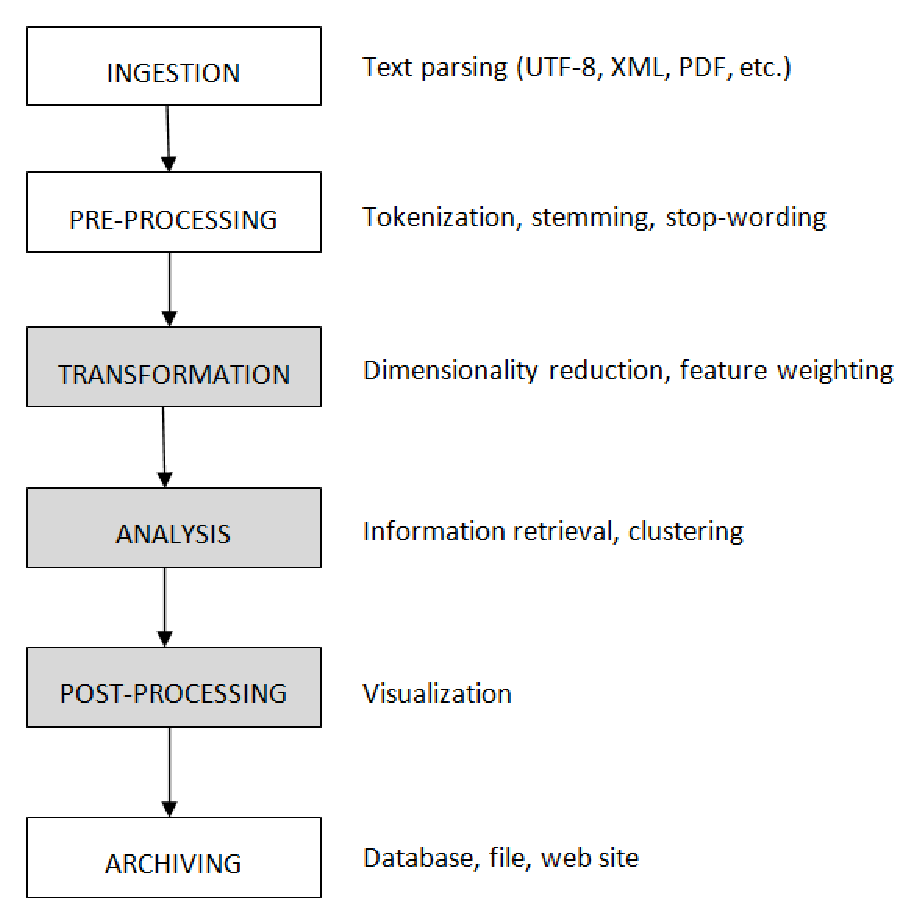
\includegraphics[width=\ScaleIfNeeded]{img/text_analysis}
%	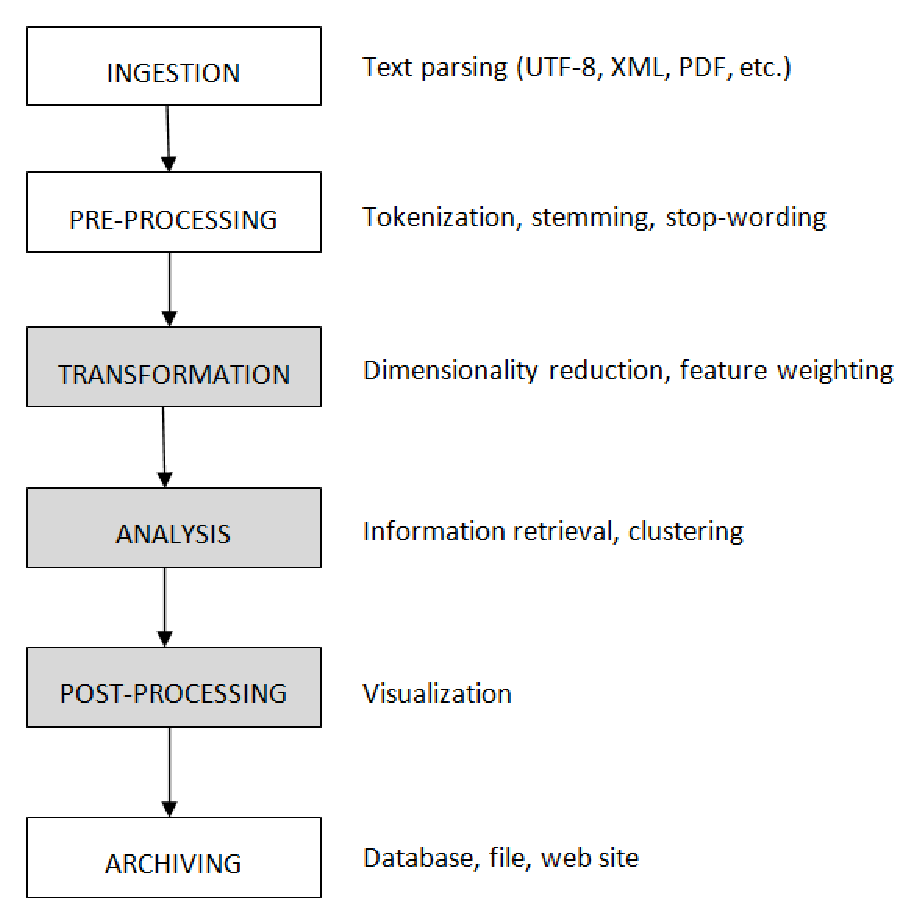
\includegraphics[width=\ScaleIfNeeded]{img/text_analysis} 
%\includegraphics[height = 0.7\textheight, trim = 30 100 30 280, clip, angle = 270]{timer}
 % or [scale=0.5]
	\caption[Workflow in IR systems]%
           {[Workflow in IR systems}
\end{figure}

The current work contributes in the transformation, analysis and post-processing phases of \gls{IR} workflow. The research focus is automatic identification of the main topics in a set of documents, returned as results to user queries. Research is done in analysis and visualization phases of the text analysis sequence diagram\ref{fig:text_analysis}. \\


This thesis contributes right here; techniques are developed which address the
design and the operationalization of IR processes respecting the above points.
The research focus is automatic document categorization, a technique which has
been shown to improve retrieval performance.\\


\section{Goal and scope of work}
This works contributes with the following:
\begin{enumerate}
\item It offers an overview of the current cluster labeling algorithms, and makes an evaluation of \gls{WCC}, proposed for unsupervised topic labeling of clusters in \cite{Stein04topicidentification} and \cite{Stein07topicidentification}.
\item It proposes an improvement in \gls{WCC} algorithm, performing topic identification based on external knowledge. A light-weight ontology has been developed for this purpose, in order to be used as a reference for external semantic knowledge during cluster labeling. 
\item A software application for executing an IR process has been developed. It implements \gls{LSA} for information retrieval, and \gls{WCC} for visualization of the main concepts contained in a document set in the form of a tag cloud. \\
\end{enumerate}


\section{Outline}
This chapter motivates the presented research work, and summarizes its contributions. It also offers a general overview to the phases of text analysis, common to most IR systems. Chapter 2 gives theoretical foundations for preprocessing and transformation phases of text analysis, and reviews a specific technique for information retrieval, called Latent Semantic Analysis. Chapter 3 contains the contribution related to evaluation of \gls{WCC} algorithm, and a proposal for its improvement, by using a light-weight ontology developed for this purpose. It represents the analytical phase in \gls{IR} systems. Chapter 4 refers to the post-processing phase of text analysis, giving the visualization means for presenting the main concepts retrieved from a document set. The software contribution, developed as a part of this work, is described in Chapter 5. Finally, in Chapter 6 the thesis concludes with evaluation of results and outlook.\\


\chapter{Latent Semantic Analysis}
\label{sec:lsa}

\begin{summary}
The chapter gives a theoretical overview of \gls{LSA} in the context of its use in this work.
\end{summary}
 
\section{Overview}
\label{sec:lsa:overview}

\gls{LSA} was first introduced in ~\cite{Dumais88usingLSA} and~\cite{Deerw90_LSA} as a technique for improving information retrieval. Most search engines work by matching words in a user's query with words in documents. Such information retrieval systems that depend on lexical matching have to deal with two problems: synonymy and polysemy. Due to the many meanings which the same word can have, also called polysemy, irrelevant information is retrieved when searching. And as there are different ways to describe the same concept, or synonymy, important information can be missed. \gls{LSA} has been proposed to address these fundamental retrieval problems, having as a key idea dimension reduction technique, which maps documents and terms into a lower dimensional semantic space. \gls{LSA} models the relationships among documents based on their constituent words, and the relationships between words based on their occurrence in documents. By using fewer dimensions that there are unique words, \gls{LSA} induces similarities among words including ones that have never occurred together~\cite{Dumais2006}. There are three basic steps to using \gls{LSA}: text pre-processing, computing \gls{SVD} and dimensionality reduction, and querying the constructed semantic space.\\
 
\section{Text pre-processing}
\label{sec:lsa:pre-processing}

If we have a document collection or a text corpus, on which we want to apply \gls{LSA}, the initial step is to pre-process the texts into a suitable form for running \gls{LSA}. Pre-processing can include a number of techniques, depending on the application requirements. The process of parsing, also called tokenization, is breaking the input text stream into useable tokens. During tokenization, filtering can be applied, i.e. removing HTML tags or other markup, as well as stop-wording, and removing punctuation marks. Stop words don't convey information specific to the text corpus, but occur frequently, such as: $ a, an, and, any, some, that, this, to $. \\

A distinction has to be made between words or terms, and tokens. A term is the class which is used as a unit during parsing, and a token is each occurence of this class. For example, in the sentence: 

\begin{quote}
\textit{CoreMedia CMS is shipped with an installation program for interactive graphical installation and configuration of the software.}
\end{quote}

the term $ installation $ is represented by two tokens. \\

There is no universal way in which to parse a text, and the parsing decisions to address depend on the application in which the text collection will be used. Text parsing will influence all posterior processing in the following stages of \gls{LSA}. \\

After tokenization, one has to construct a term-document matrix~(\ref{lsa:sparse_matrix_A}). Having as rows the terms, and as columns the documents, its elements are the occurrences of each term in a particular document, where $ a_{ij} $ denotes the frequency with which term $ i $ occurs in document $ j $. The size of the matrix is \text{\bf{m x n}}, where {\bf m} is the number of terms, and {\bf n} is the number of documents in the text collection. Since every term doesn't appear in each document, the matrix is usually sparse. \\

%
% initial sparse matrix A
%
\begin{equation}
A=
\begin{bmatrix}
\label{lsa:sparse_matrix_A}
 a_{11}& a_{12}& \cdots& a_{1n} \\
 \vdots& \vdots& \ddots& \vdots \\ 
 a_{m1}& a_{m2}& \cdots& a_{mn}
\end{bmatrix}
\end{equation}\\

Local and global weightings are applied to increase or decrease the importance of terms within documents. We can write
%
% general weighting function
%
\begin{equation}
\label{lsa:global_local_weighting}
a_{ij}=L(i,j) \times G(i),
\end{equation}

where $L(i,j)$ is the local weighting of the term $i$ in document $j$, and $G(i)$ is the global weighting for term $i$. The choice of a weight function has impact on \gls{LSA} performance, therefore in Section~\ref{sec:lsa:factors_infl_lsa} we give an overview of the most common weight functions. \\

\section{Singular Value Decomposition}
\label{sec:lsa:svd}

After the initial pre-processing, the term-document matrix is decomposed into three matrices~(\ref{lsa:svd}) by applying Singular Value Decomposition~(\gls{SVD}). It is a unique decomposition of a matrix into the product of three matrices - $U$ and $V$ are ortonormal matrices, and $ \Sigma $ is a diagonal matrix having singular values on its diagonal.\\
%
% SVD decomposition in three matrices
%
\begin{equation}
\label{lsa:svd}
A=U \Sigma V^{T}
\end{equation}\\

After the initial matrix $A$ is decomposed, all but the highest $k$ valued of $S$ are set to $0$. The resulting reduced matrix is the semantic space of the text collection. A classical example presenting the truncated \gls{SVD}~\cite{Dumais88usingLSA}  can be used for displaying dimensionality reduction, and how it affects all three matrices.\\
%
% diagram of the truncated SVD
%
\begin{center}
\begin{figure}[htbp]
\label{lsa:truncated_svd}
	\centering
	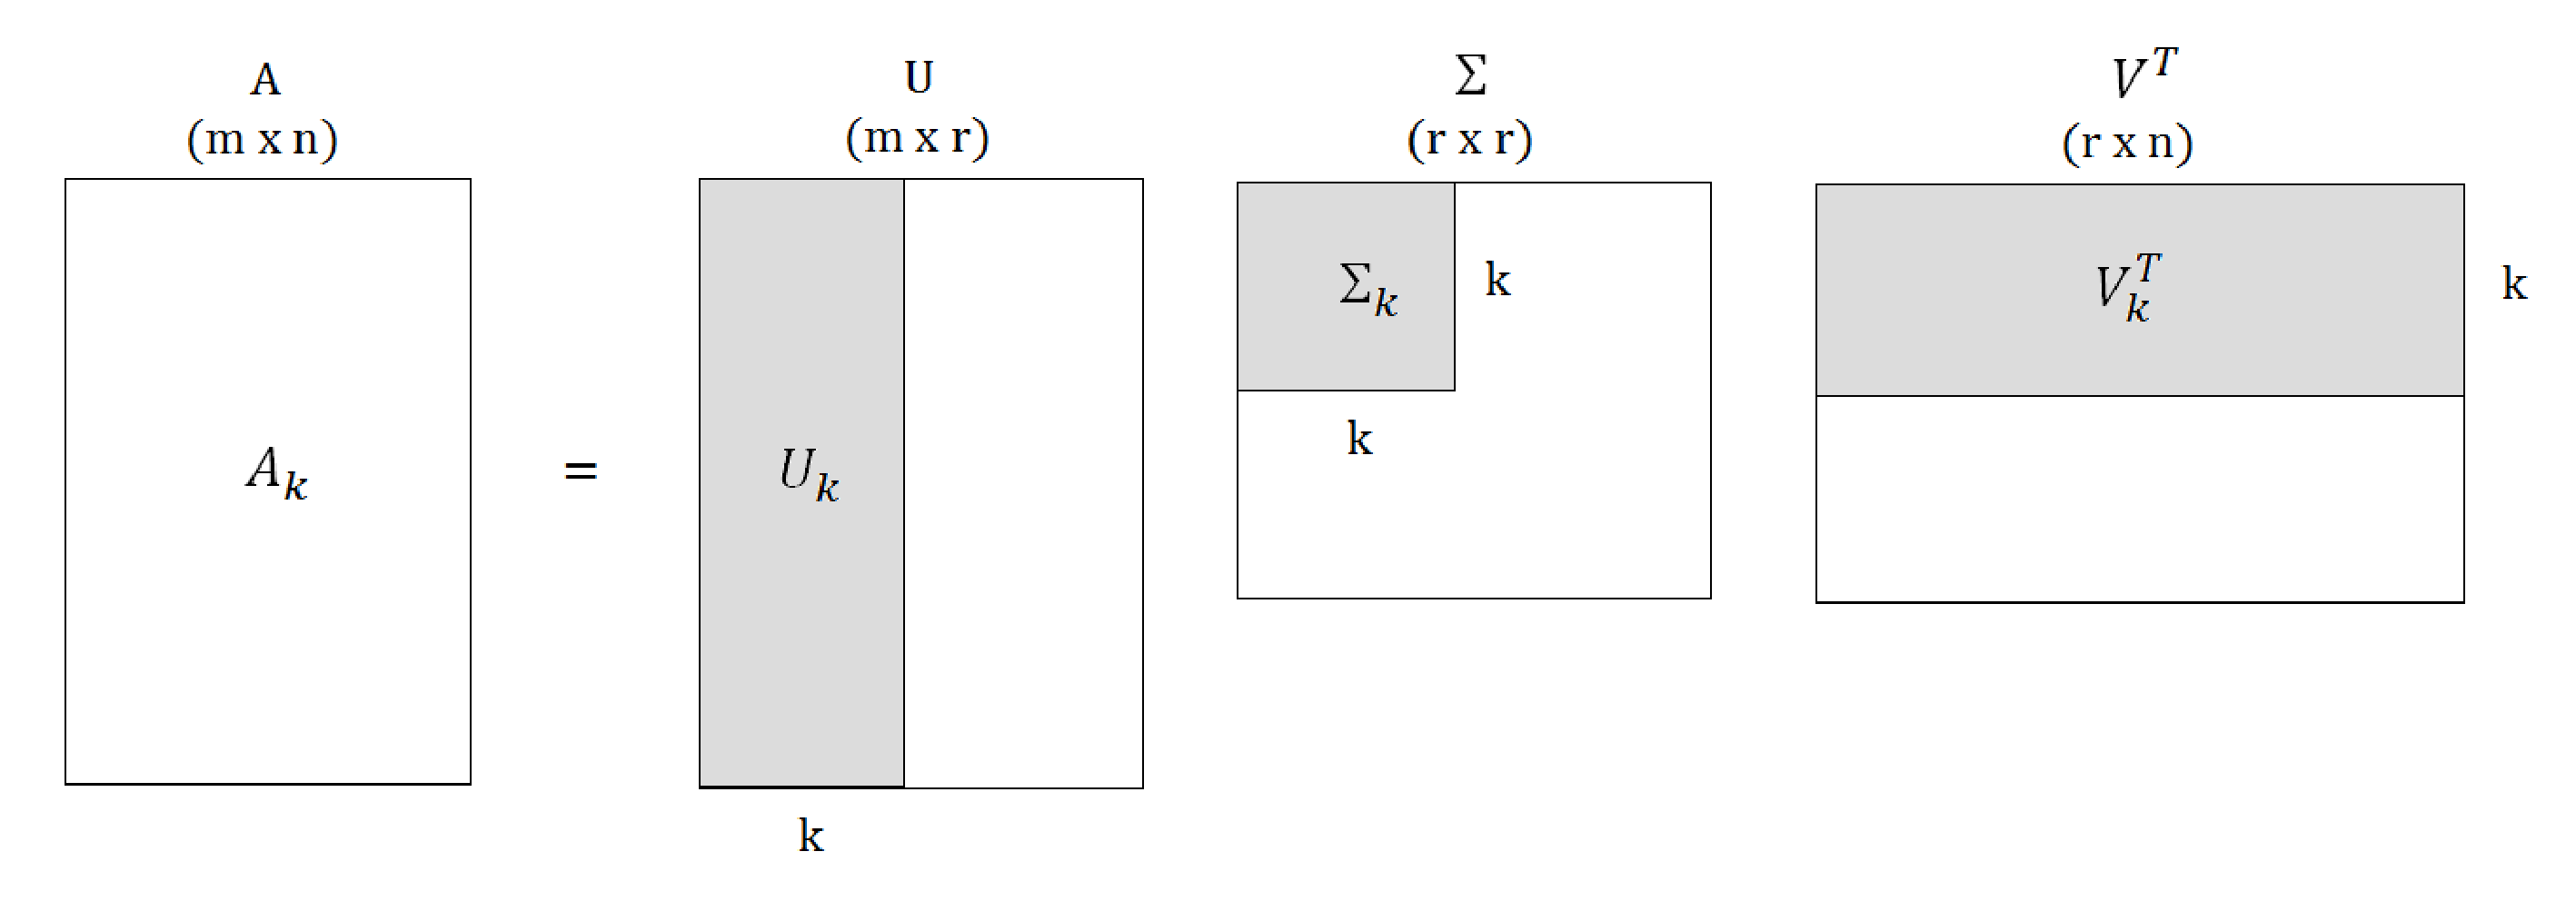
\includegraphics[width=\ScaleIfNeeded]{img/svd} 
 % or [scale=0.5]
	\caption[Diagram of truncated SVD]%
           {Diagram of truncated SVD}
\end{figure}
%
% description of the parameters in SVD diagram
%
\begin{tabular}{l l}
$A_{k}$ - best rank-$k$ approximation of $A$ & $m$ - number of terms\\
$U$ - term vectors & $n$ - number of documents \\
$\Sigma$ - singular values & $k$ - number of factors \\
$V^{T}$ - document vectors & $r$ - rank of $A$ \\
\end{tabular}
\end{center} 

Figure~\ref{lsa:truncated_svd} is a visual representation of \gls{SVD} as defined in equation~(\ref{lsa:svd}). $U$ and $V$ are considered as containing the term and document vectors respectively, and $\Sigma$ is constructed by the singular values of $A$. An imporant property of \gls{SVD} is that the singular values placed on the diagonal of $\Sigma$ are in decreasing order. Hence, if all but the first $k$ singular values are set to $0$, the semantic meaning in the resulting space is preserved to some approximation $k$, while noise or variability in word usage, is filtered out. Noise in this case are the terms with lowest weights which carry little meaning. By using fewer dimensions $k$, \gls{LSA} induces similarities amont terms including ones that have never occured together. Terms which occur in similar documents, for example, will be near each other in the k-dimensional space even if they never co-occur in the same document. This means that some documents which do not share any words with a users query may be near it in k-space.\\

A factor to be considered when computing \gls{SVD} is the run-time complexity of the algorithm. For decomposition of very large matrices, it is $O(n^2k^3)$, where $n$ is the number of terms in the text corpus, and $k$ is the number of dimensions in semantic space after dimensionality reduction. Note that $k$ is typically a small number between 50 and 350.\\

A more detailed description of \gls{SVD} can be found in \cite{Berry95usinglinear} and \cite{MatrixCompGolub96}.\\

\section{Querying the semantic space}
\label{lsa:querying_sspace}

In this work we are using \gls{LSA} for \gls{IR} purpose. Therefore, the final step of applying the technique is to pose queries on the constructed semantic space. A query $q$ is a set of words which must be represented as a document in the k-dimensional space, in order to be compared to other documents. The user's query can be represented by
%
% Query translation for LSA
%
\begin{equation}
\label{lsa:query}
q = q^{T}U_{k}\Sigma_{k}^{-1}
\end{equation}\\
where $q$ is the set of words in the query, multiplied by the reduced term and singular values matrices. Using the transformation in~(\ref{lsa:query}), the query is ''mapped'' onto the reduced k-space. After the mapping, the resulting query vector can be compared to the documents in the k-space, and the results ranked by their similarity or nearness to the query. A common similarity measure is the cosine between the query and the document vector. From the resulting document set, the documents closest to the query above certain treshold are returned. \\

\section{Factors influencing LSA performance}
\label{sec:lsa:factors_infl_lsa}
The effective usage of \gls{LSA} is a process of a sophisticated tuning. Several factors can influence the performance of the technique. These factors are pre-processing of texts~(removal of stop-words, filtering, stemming), frequency matrix transformations, choice of dimensionality $k$, choice of similarity measure.\\

Dumais et al.~\cite{dumais91improving} and Nakov et al.~\cite{Nakov_weightfunctions} have carried research on \gls{LSA} performance depending on the choice of factors such as frequency matrix transformations, similarity measures, and choice of dimension reduction parameter $k$. They conclude that performance based on the choice of these factors depends on the particular text corpus, as well as on the purpose of \gls{LSA} application. However, in the case of matrix transform, log-entropy performs better as compared to other matrix transform function combinations, including the popular term frequency - inverse document frequency~($tf\times idf$). Therefore, we implement the former in this work.
%
% entropy frequency matrix transformation
%
\begin{center}
\begin{tabular}{l l}
Local function:  & \multirow{2}{*}{ $ L(i,j)=\log(tf(i,j)+1) $ }\\
logarithm & \\
Global function: & \multirow{2}{*}{ $ G(i)=1+\frac{{\Sigma_{j}p(i,j)}}{\log n} $ } \\
entropy & \\
\end{tabular}
\end{center} 
where $n$ is the number of documents in the collection.\\

Further, it has been stated~(\cite{dumais91improving},\cite{NakovBetterResultsLSI}) that with respect to similarity measures used, \gls{LSA} performs optimal when cosine similarity measure is implemented to calculate the distance between vectors in the semantic space. We have therefore used it to measure the relevance between queries and documents. The cosine measure between two vectors $d_1$ and $d_2$ is given by:
%
% cosine similarity
%
\begin{equation}
\label{lsa:cosine_measure}
sim(d1,d2)=\frac{\overrightarrow{V}(d_1).\overrightarrow{V}(d_2)}{\left\vert \overrightarrow{V}(d_1) \right\vert.\left\vert \overrightarrow{V}(d_2)\right\vert}
\end{equation}

Dimensionality reduction parameter $k$ is defined empirically based on the experimentation results presented in Chapter~\ref{sec:implementation}. 

\chapter{Tag Clouds}
\label{sec:tagclouds}

Tagging, which is one of the defining characteristics of Web 2.0 services, allows users to collectively classify and find information. Some websites include tag clouds as a way to visualize tags in a folksonomy.(4)\\

An empirical analysis of the complex dynamics of tagging systems, published in 2007,(5) has shown that consensus around stable distributions and shared vocabularies does emerge, even in the absence of a central controlled vocabulary.For content to be searchable, it should be categorised and grouped. This is possible only if the content is tagged like keywords in a journal article.\\

(4) Lamere, Paul (June 2008). "Social Tagging And Music Information Retrieval". Journal of New Music Research 37 (2): 101�114. http://www.informaworld.com/smpp/content~db=all~content=a906001732. \\
(5) Harry Halpin, Valentin Robu, Hana Shepherd The Complex Dynamics of Collaborative Tagging, Proceedings of the 16th International Conference on the World Wide Web (WWW'07), Banff, Canada, pp. 211-220, ACM Press, 2007. \\

We have found so far no other application implementing LSA in order to present an overview of the main topics found in a collection of unstructured texts, based on user queries. The TagCloud Summarizer is in this sense new.\\

There exist, however, search engines, which utilize categorizing of search results, such as Yippy(former Clusty, Vivisimo). It utilizes search, classification, and Social web (Web 2.0).
\section{existing implementations}
http://cloud.yippy.com/  - visualizes topics based on search queries. Created at Vivisimo company, also creator of one of the most successful meta search engines, offering classification of search results, Clusty (Vivisimo). \\

SenseBot Summarizer summarizes search results in the form of a tag cloud.\\

Google on the other hand offers "Wonder wheel" option, in order to display search results \\ 

TagCloud Summarizer is a tool that users can use to instantly visualize a topic using the familiar tag cloud display. Users can create a cloud based on a query.\\

TagCloud Summarizer generates a cloud using the user's search results for the topic they enter. Using the Summarizer to generate the cloud also ensures that it is always up-to-date because topics/main concepts are generated in real-time, based on the user's query.\\

\section{use}
Use the TagCloud Summarizer for online web-pages, search systems, or personal web-sites.\\

\begin{summary}
This chapter presents an overview of tagclouds used as a method for representing text content.
\end{summary}

Tag Clouds are popular applications used for vaious purposes: as a navigation mechanism, as indicators of activity within social media experiences, for visualization in texts and textual data, for annotation of documents~\ref{fig:tagcloud}. The importance or weight of words in the tag cloud are shown with size of font and/or color. The tag clouds are hyperlinks leading to a collection of items associated with the tag.\\
A version of tag cloud is called text cloud. It is used as a visual display that conveys the broad themes that emerge from textual analysis.  
There are three types of tag clouds depeding on their purpose and use. The first type contains a tag represeting the frequency of each term. The second type is a global tag cloud whose tags has frequencies aggreggated over all items and users. The third type of tag cloud contains categories, and its tags' size indicates the number of subcategories.\\
%TODO
%generate a tag cloud based on the contents in docmachine!!!!!!! replace the figure
%
% Opencloud
%
\begin{figure}[htbp]
	\centering
	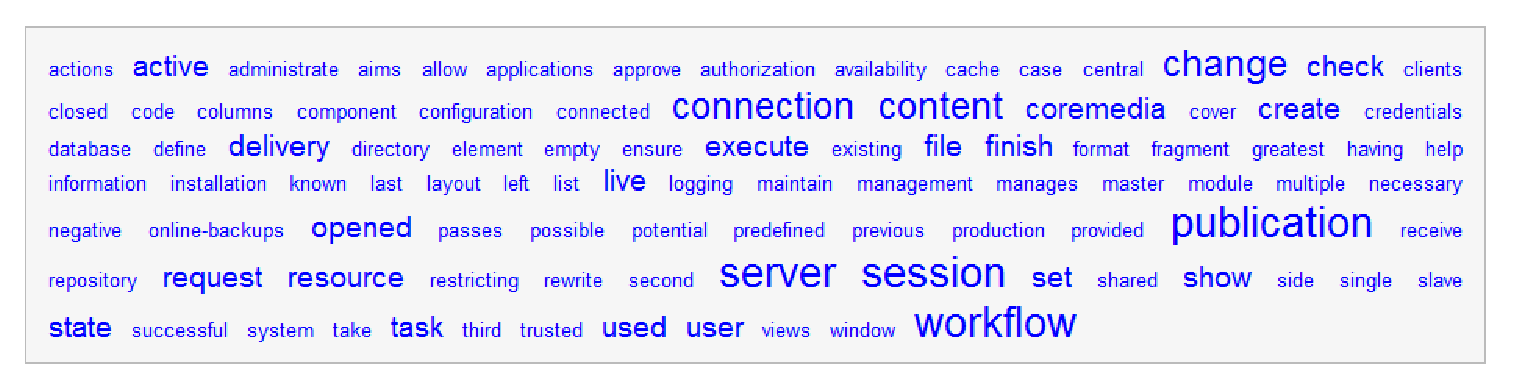
\includegraphics[width=\ScaleIfNeeded]{img/tagcloud} 
 % or [scale=0.5]
	\caption{Tag Cloud}
	\label{fig:tagcloud}
\end{figure}

\section{1}
\label{sec:semannot:1}
Related work \\
Opinion Crawl\footnote{\url{http://www.opinioncrawl.com/}} - web sentiment analysis application. It generates a concept cloud from daily scanned blogs, web site articles. \\

SenseBot Search Results Summarizer is a plugin for Mozilla Firefox browser that generates a tag cloud of the main concepts returned as search results from Google. \\

Search Cloudlet\footnote{\url{https://addons.mozilla.org/en-US/firefox/addon/9943/}} is another Firefox Addon that inserts a related tagcloud into Google interface. Working behind the scenes, Search Cloudlet injects a tag cloud of related words in to both Google and Yahoo search results pages. Then you can use the tag links to quickly and easily filter and refine your searches.



LinkSensor
SenseBotSummarizer
All three are based on SenseBot - a semantic search engine.
Made available from Semantic Firefox Extensions \footnote{\url{http://www.semanticengines.com/plugins.htm}}\\

\section{Brainstorming}
What is a tag cloud? Graphical representation of a collection of tags. Tag clouds visualize word frequency in a given text.\\

Tag clouds may be used as a topic summary.\\

There are three main types of tag cloud applications used in social software.\\
\begin{enumerate}
\item frequency of items / tags
\item number of items to which a tag has been applied
\item tags are categorization method for content items 
\end{enumerate}
The following tag clouds were evaluated in order to select the solution that is most applicable for Tag Cloud Summarizer project.\\
\begin{itemize}
\item Yippi Cloud Creator (former Clusty) \footnote{\url{http://cloud.yippy.com/}}
\item TagsTreeMaps\footnote{\url{http://tagstreemaps.sourceforge.net/TagsTreeMaps.html}}
\item OpenCloud\footnote{\url{http://opencloud.sourceforge.net/}}
\end{itemize}

\section{Tag clouds construction}
According to \cite{hoppe:2010}: \\
Erstellung von Schlagwortwolken
Tagging beschreibt die Aktivit�t, eine Ressource mit einem oder mehreren Schl�sselworten
oder Schl�sselphrasen zu assoziieren. Ein Tag ist als Etikett oder Notiz zu verstehen,
um zu einem sp�teren Zeitpunkt Dinge leichter wieder finden zu k�nnen. Tags dienen
somit der Organisation von Ressourcen.
Gro�er Beliebtheit erfreuen sich unter anderem kollaborative Tagging-Dienste wie
Flickr (Bilder), del.icio.us (Internetseiten) oder Facebook (soziales Tagging). Beim kollaborativen
Tagging annotieren Nutzer selbst die entsprechenden Ressourcen. Der auf diese
Weise implizit entstehende sogenannte tagspace soll anschlie�end effizient durchsuchbar
sein. Jedoch f�hrt das manuelle Annotieren von Ressourcen zu Problemen, wie Golder
u. Huberman (2006) aufzeigen. Synonyme und Polyseme verursachen dabei Probleme,
die bereits in Kapitel 2.1.1 angesprochen wurden. So schlie�t eine Bildersuche mittels
des Schl�sselworts Auto keine Bilder mit ein, die nur mit dem Synonym Pkw assoziiert
sind. Ein weiteres Problem ist, das dieselben Ressourcen von verschiedenen Nutzern unterschiedlich
annotiert werden. F�gt ein Nutzer als Schl�sselwort einem Bild Auto als
Schl�sselwort hinzu, so wird ein anderer durch Zuweisung von Volkswagen Golf Mk5
(A5/Typ 1K, 2003-2009) deutlich konkreter.
Um Inkonsistenzen bei der Zuweisung von Tags zu vermeiden und dadurch die Retrievalqualit�t
von Suchmaschinen zu steigern, wird automatisches Tagging eingesetzt.
Dieses dient vor allem beim Annotieren von neuen Weblog-Nachrichten dazu, Empfehlungen
f�r passende Schl�sselworte einem Nutzer vorzuschlagen.
Brooks u. Montanez (2006) annotieren automatisch neue Nachrichten in Weblogs. Sie
verwenden dazu die drei h�ufigsten Terme einer Nachricht, gewichtet nach dem tf-idf -
Schema. Nachteil ist, dass Schl�sselworte somit auf Wort-Unigrammen und dem der
Nachricht zugrundeliegenden Vokabular beschr�nkt sind.
Mishne (2006) ermitteln zu neuen Nachrichten in Weblogs zun�chst �hnliche Nachrichten,
die von anderen Nutzern zuvor verfasst wurden. Anschlie�end werden einem Nutzer
die dort verwendeten Schl�sselworte als Tags f�r eine neue Nachricht vorgeschlagen.
Lee u. Chun (2007) setzen dagegen ein �berwachtes Lernverfahren ein � ein neuronales
Netz. Dieses wird auf einer Menge von Blog-Nachrichten trainiert, denen Tags zugewiesen
sind. Anschlie�end k�nnen Empfehlungen f�r Tags f�r neue Nachrichten gegeben werden.
Grundlage zur Erfassung von Tags sind Verfahren der Schl�sselwortbestimmung. Dabei
werden h�ufige, durch tf-idf gewichteteWort-Bigramme in den Nachrichten ermittelt. Ob
die ermittelten Bigramme auch allgemein h�ufig verwendet werden, wird anschlie�end
mittels WordNet evaluiert.
Neben der automatischen Empfehlung von Schl�sselworten wird ebenso versucht, aus
dem tagspace eine Hierarchie abzuleiten (Brooks u. Montanez, 2006; Wu u. a., 2006).
Solche Hierarchien dienen der Suchoptimierung. Da im Allgemeinen bei der Erstellung
von Schlagwortwolken auf vorhandene Schl�sselworte zur�ckgegriffen wird, finden sich
bis auf die Erstellung von Taxonomien aus Schlagworten keine Gemeinsamkeiten mit
Ans�tzen des Cluster-Labelings. 


\chapter{Implementation}
\label{sec:implementation}

This chapter describes the implementation part of the thesis work. After presenting in Chapter~\ref{sec:lsa} the theoretical basis behind \gls{LSA}, and in Chapter~\ref{chapter:cluster_labeling} cluster labeling, theoretical application and specific implementation decisions are discussed here. All software tools and libraries which were used are pointed out, and code snipplets are given. Then in Chapter~\ref{chapter:evaluation}, test results are shown, and evaluation of the implementation is made. \\


\section{Tag cloud summarizer}

The prototype implementation is a web application, which outputs a tag cloud based on users' queries. Initially, a preprocessing of the document set is done, then a semantic space is constructed by running \gls{LSA} and performing dimensionality reduction during \gls{SVD}~(refer to Chapter~\ref{sec:lsa} for the terminology). The initial two stages are performed offline. Once the document set is indexed by a term-document  matrix, queries can be made by users. The terms in the documents closest to the queries in the semantic space, are input to the tag cloud. Querying and tag cloud generation are performed interactively online. \\

The desicion to implement the prototype as a web application is due to two factors. Firstly, tag clouds are widely spread in online systems, and thus mainly used online. And secondly, the prototype should be implemented in the online documentation system DocMachine\footnote{\url{https://documentation.coremedia.com/}} at CoreMedia AG, Hamburg, and should also be available online. \\

\subsubsection{Preprocessing}
The documents used for evaluation are a part of the online documentation at CoreMedia AG, Hamburg\footnote{\url{https://documentation.coremedia.com/}}. Documents are stored as XML files, and CoreMedia \gls{CMS} Unified API\footnote{\url{https://documentation.coremedia.com/servlet/content/241548?language=en&version=5.2&book=coremedia:///cap/content/241548}} is used to access the plain text, as shown in Listing~\ref{doc_preprocessing}. Before executing \gls{LSA}, a preprocessing the text corpus is made, in order to construct a semantic space from a document collection. Stop words, puncutuation and numbers are removed. No stemming is done, as terms from the semantic space are later used for a tag cloud generation. 

\subsubsection{LSA}
The LSA implementation uses an opensource Java-based library, called S-Space (see section~\ref{sec:implementation:tools_used}). Partial code for \gls{LSA} is given in listing~\ref{code_lat_analysis}. The complete source code can be found in the online repository where this work in available online\footnote{\url{https://github.com/angievelinska/Tag-Cloud-Summarizer/tree/master/summarizer/src/main/java/edu/tuhh/summarizer/lsa}}).

\subsubsection{Querying the semantic space}
After the semantic space has been constructed, and dimensionality reduction has taken place, queries can be made to find the documents closest to a given query, or the terms respectively, by querying the documents or term space. As a reminder, the term space consists of the matrix product: $U * \Sigma$, and the document space of the product: $\Sigma * V^{t} $ (fig.~\ref{lsa:truncated_svd}). 
In listing~\ref{querying} the source code for querying the semantic space is given.

\subsubsection{Tag cloud generation}
A tag cloud is generated using a collection of terms (or tags) with their corresponding weights. The weights are just the normalized term frequencies after a dimensionality reduction took place during \gls{LSA}. In listing~\ref{tag_cloud} is given the source code used for generating the tag cloud. \\

The Tag cloud summarizer is a tool that should aid the users of an \gls{IR} systems obtain a quick overview of the main concepts contained in search results they receive. As it will be used by users, its evaluation should in the best case be made by them. In Chapter~\ref{chapter:evaluation} is provided a simple evaluation of the Tag cloud summarizer based on user feedback. 

\section{Cluster labeling}
The algorithm for cluster labeling Weighted Centroid Covering is implemented in Java. It receives as input predefined clusters, and nominates cluster labels for each cluster. A detailed overview of the algorithm can be found in section~\ref{clustering:WCC}. A part of the source code  of this algorithm can be found in listing~\ref{topic_identification}.

\section{Tools and libraries used in this work}
\label{sec:implementation:tools_used}

\subsubsection{Repository}
This thesis work is available online hosted in a reporitory under GitHub. Prototype implementation\footnote{\url{https://github.com/angievelinska/Tag-Cloud-Summarizer}}, project report\footnote{\url{https://github.com/angievelinska/Tag-Cloud-Summarizer/raw/master/report/thesis.pdf}} and \LaTeX~template\footnote{\url{https://github.com/angievelinska/Tag-Cloud-Summarizer/tree/master/report}} can be downloaded freely. \\

\subsubsection{LSA and SVD}
In this work the popular SVD C library\footnote{\url{http://tedlab.mit.edu/~dr/SVDLIBC/}, accessed December, 2010}  is used, created by Doug Rohde at the Massachusetts Institute of Technology. The implementation developed as a part of this project is Java-based, therefore for matrix computations the open source SVDLIBJ\footnote{\url{http://bender.unibe.ch/svn/codemap/Archive/svdlibj/}, accessed December, 2010} library is used, which is a Java-based port of SVD C, made available by Adrian Kuhn and David Erni at the University of Bern. \\

\subsubsection{k-means clustering algorithm}
Cluto clustering library\footnote{\url{http://glaros.dtc.umn.edu/gkhome/cluto/cluto/overview}, accessed October, 2010} is used as an implementation of the k-means clustering algorithm.\\

\subsubsection{Information retrieval}
S-Space project created by  Jurgens and Stevens~(\cite{S-Space}) was used for constructing a semantic space from the document set used for evaluation. \\

\subsubsection{Tag cloud}
The tag cloud used in this work is based on Opencloud\footnote{\url{http://opencloud.mcavallo.org/}, accessed December, 2010} project, authored by Marco Cavallo.\\

\subsubsection{Search and retrieval of search results}
Lucene\footnote{\url{http://lucene.apache.org/java/3_0_2/}, accessed December, 2010} is an open source search engine library, distributed by the Apache Software Foundation. It is used for indexing, query parsing and retrieval of search results. \\

\subsubsection{CoreMedia CMS domain ontology}
For the ontology development, Protege Ontology Editor 4.1\footnote{\url{http://protege.stanford.edu/}, accessed December, 2010} was used, developed at Stanfornd University. The ontology is a light-weight domain ontology developed in OWL for CoreMedia \gls{CMS} domain (Appendix~\ref{appendix:onto} and listing~\ref{cm_ontology}). \\


\subsubsection{Building and deployment}
Maven\footnote{\url{http://maven.apache.org/}} is a software management tool, provided by Apache Software Foundation, which is used for building and testing the implementation prototype, and for deploying the web application module.



\chapter{Conclusion and outlook}
\label{sec:conclusion}

\begin{summary}
summarize me
\end{summary}

\section{1}
\label{sec:conclusion:1}

\section{Future Work}
\begin{enumerate}
\item implement LSA based IR in full-text search results, or as recommendation.
\item link tags from tag cloud to the documents where they occur (using lucene indexing ???)
\item investigate also the case of updating the document collection - how to handle this case
\item Improve TagCloudSummarizer to work also with German texts (company has a website that support German, Russian, French..)
\item Make the process run in parallel.
\end{enumerate}


% prints the list of acronyms
% call: latex thesis, makeglossaries thesis, latex thesis
%
\printglossaries


\begin{appendix}















\chapter{Appendix}

TODO: insert important source code parts here.

\end{appendix}

% After adding new references to the "references.bib" file, first invoke latex, then
% bibtex on the references file, then latex again:
% latex thesis
% bibtex thesis
% latex thesis

% number the bibliography instead of alpha-numerial abbrev.
%\bibliographystyle{alpha} 
\bibliographystyle{ieeetr}
\bibliography{references}
\end{document}
